\documentclass[11pt,conference]{IEEEtran}
\title{Promiscuous Speculation: When is it inappropriate to flaunt your guesses?}
\author{William Wesley \\
\texttt{wwesley@uccs.edu} \\
University of Colorado \\
Colorado Springs, Colorado}

\usepackage[T1]{fontenc}
\usepackage{graphicx}
\usepackage{listings}
\usepackage{xcolor}
\usepackage{mathtools}

\definecolor{codegray}{rgb}{0.5,0.5,0.5}

\lstdefinestyle{mystyle}{
    numberstyle=\tiny\color{codegray},
    basicstyle=\ttfamily\footnotesize,
    breakatwhitespace=false,
    breaklines=true,
    keepspaces=true,
    numbers=left,
    numbersep=5pt,
    showspaces=false,
    showstringspaces=false,
    showtabs=false,
    tabsize=2,
    frame=lines,
    xleftmargin=10pt,
    xrightmargin=10pt,
    literate=
       {->}{$\rightarrow{}$}{1}
       {<-}{$\leftarrow{}$}{1}
}

\lstset{style=mystyle}

\begin{document}

\maketitle

\begin{abstract}
Lalalal...
\end{abstract}

\section{Introduction}

Speculative execution attacks have rightfully garnered much attention in the past few years.
With the publication of the Meltdown\cite{meltdown} and Spectre\cite{spectre} vulnerabilities in 2018 and 2019, respectively, the public became acutely aware of some promiscuous behaviors undertaken by modern processors in the name of performance.
These behaviors lead directly to compromises in system security by violating the abstraction between hardware and software.

However, the performance gains obtained by speculative execution are so great that we refuse to abandon it and instead seek to mitigate the vulnerabilities in a combination of hardware and software patches.
We reduce the fidelity of side-channels to deteriorate the performance of attacks to the point that there is more likely an easier way to compromise the system elsewhere.
We prevent access to sensitive areas of memory by obscuring their location or confining speculative accesses.
We disable speculative execution with ``fences'' that are software instructions that force the processor into taking more care in particularly risky code structures.

However, reducing precision for legitimate computations limits the usefulness of timers, strategies to confine or obscure memory access can make code more difficult to understand and therefore more prone to containing bugs, and littering code with fences to prevent speculation will limit the performance benefits of doing speculation in the first place.
So, how can we defend against speculative attacks without unnecessarily sacrificing precision, performance, and readability?
How can we identify where the risks are so we can balance these conflicting needs?

In \S\ref{sec:background} we discuss what speculative execution attacks are and what enables them.
In \S\ref{sec:related} we talk specifically about work modelling software to identify ``gadgets,'' which can be used to identify places in software where fences or access confinement are necessary to ensure system security.
Then in \S\ref{sec:future} we identify potential avenues for future research in this area.

\section{Background}\label{sec:background}

Modern general purpose processors derive a large part of their performance from ``speculative execution.''
Control-flow-affecting instructions present a problem to performance in that the information required to make a control flow decision may not be available before the decision must be made.
Waiting for that information will result in delays and degradation of system performance.
However, if the system can accurately predict\footnote{That is, guess better than a coin flip.} the decision, then it can begin execution of the instructions in the correct flow of control before that decision can be made.
Any uneasiness with this proposal is calmed with the promise that if the prediction is incorrect, the system can simply ``roll-back'' the effects of the incorrect control flow and the penalty for doing so will not be much more than if the system waited for all the information.
In this way, we optimize for the common case where our predictions are correct and accept some penalty in the rare case that our predictor fails us.

Another tool employed, in many variations, to increase system performance is \emph{caching}.
We will define caching in this paper as any memory structure that is used to avoid repeating previous work.
For example, a request to main memory can be cached so that if the same request is repeated, it can be satisfied from the cache rather than a whole new request to main memory.
Similarly, a translation from virtual memory to physical memory can be saved in a cache so that next time the operating system need not be invoked to perform the translation.
Yet another example is fast memory locations built into larger memory components that store the results of recent requests to the component, such as row buffers in main memory or cache memory on a disk drive.
In all of these cases, temporal and physical locality is exploited to reduce the time required to complete execution of a program by avoiding the performance on all of the ``movements'' that would be strictly required.

But, variations in performance are exactly the kind of behavior that lead to Timing Attacks as described by Kocher over twenty-five years ago\cite{kocher96}.
If the system performance varies with the input of some secret value, that value can potentially be inferred from that variation - that is the variation in time is a ``side-channel'' to obtaining the secret that the software developer may or may not have accounted for in constructing the system.
Caching alone provides this potential side-channel\cite{shepherd2022transient}, but when combined with speculative execution, the risk is amplified.

In a system with cache in place, the results of a computation or other activity are available quicker if those results were recently obtained.
In one approach, an attacker might cause a series of computations to be performed and compare the relative times to identify which computation was recently performed, thus identifying which one was executed by the victim and uncovering potential secrets.
Such an attack would be expensive, but still possible.
With speculative execution, if an attacker can cause the predictor to make an incorrect prediction while influencing what the incorrect control flow instructions do, the attacker can side step controls such as bounds checking or privilege levels in a brief window within which cache states can be affected in a relatively precise manner.

Furthermore, as Shepard, Brookes, and Denz\cite{shepherd2022transient} remind us, memory access timing is not the only side channel that might be present.
Speculative execution may also leak information in terms of varying power consumption or EM radiation.
\emph{Any} side effect changes the state of the system and potentially can be used to exfiltrate sensitive data.

Exact details vary from variant to variant of speculation attack, so for this paper we will summarize the vulnerability as situations in which speculative execution causes changes in state that is not rolled back.
Although this vulnerability is ostensibly a hardware problem since it is the processor making the decision to violate program order and execute software instructions ``on a guess,'' there are software structures that are more susceptible to falling victim to these kinds of attacks and we can mitigate the risk by modifying our code, masking our data, or explicitly instructing the processor to forego speculation.
These code structures are called \emph{gadgets} in the literature.

Consider the code snippet below, reproduced from \cite{spectre}.
\begin{lstlisting}
  if (x < array1_size)
    y = array2[array1[x] * 4096];
\end{lstlisting}
Assuming an attacker can control the value of the variable \texttt{x}, then the attacker can train the branch predictor to execute the access relative to \texttt{array1} which will allow an out-of-bounds access to speculatively execute.
The value so accessed will then be used to access data relative to \texttt{array2}, but scaled so that values map to separate cache lines.
Then the attacker can scan \texttt{array2}, timing the accesses, and by identifying which cache line returned fastest infer what the value was at the original out-of-bounds access.
This is the original gadget example from the Spectre paper but many more variations are possible.

Our main interest in this paper is how to identify these gadgets programmatically so that we can defend against attack in software.



\section{Related Work}\label{sec:related}
For this paper, we considered primarily three works which we discuss below.
We sought to understand the state of the art in defenses against speculative execution attacks and narrowed our focus on techniques to systematically identify vulnerable code.

\subsection{Defense Classification}
In \textit{A Systematic Evaluation of Transient Execution Attacks and Defenses}, Canella et al\cite{canella2019} describe Spectre and Meltdown as \emph{transient} execution attacks, that is they characterized the vulnerabilities as being the result of instructions being executed and then rolled back.
This is slightly broader than our definition in that we've focused specifically on speculative execution, whereas the transient definition would allow for instructions rolled back for some other reason than an incorrect prediction.
For example, instructions following one that creates a fault late in a pipeline may affect system state and not be the fault of a misprediction but just the normal flow of the program.
However, in a sense this is still a form of misprediction on the part of the compiler or software developer, so we chose to use the traditional nomenclature for our paper.
Their systematic evaluation of Spectre and Meltdown style attacks allowed them to formulate a classification system.
They were able to use this system to give more descriptive names to attacks that were currently known and also to identify several new attack variations.

Since Canella et al distinguish between Spectre type and Meltdown type vulnerabilities as being caused by speculation or fault, respectively, it is natural for them to classify the defenses along the same lines.
For Spectre, they give three categories of defense, paraphrased here:
\begin{enumerate}
	\item[\textbf{C1:}] Reducing the fidelity of covert channels, for example by adding jitter to or reducing the precision of timer related functions,
	\item[\textbf{C2:}] Inhibiting speculation when sensitive data might be accessed, for example placing \texttt{fence} instructions around potential gadgets, or
	\item[\textbf{C3:}] Ensuring sensitive data cannot be reached, for example masking values used in offsets can affect limits on the range available to out-of-bounds accesses in a gadget.
\end{enumerate}

For Meltdown, they divide the defenses into the following two categories:
\begin{enumerate}
	\item[\textbf{D1:}] Ensuring sensitive data cannot be reached, for example by storing such data in uncacheable memory or structures that are always sanitised on context switches, or
	\item[\textbf{D2:}] Preventing faults from occurring, for example an access to a protected page from an unprivileged mode might return invalid values instead of triggering a fault.
\end{enumerate}

For categories C2, C3, and D1, the mitigation relies heavily on the software author to balance the security concern with the performance penalty.
Simply sprinkling code with fences anywhere speculative execution may occur reduces program performance.
Failing to protect a single instance where speculation leads to exfiltration leaves the entire application insecure.
But, if we can identify gadgets programmatically, we will be better equipped to write secure and performant code.

\subsection{Leakage Containment Models}

\textit{Axiomatic Hardware-Software Contracts for Security}\cite{mosier2022} presents a model for analysis of software to detect "microarchitectural leakage" automatically.
Building on Memory Consistency Models (MCMs), Mosier et al define Leakage Containment Models (LCMs) which are used to detect gadgets and other forms of data leakage in examples from other papers.
They go on with a discussion of CLOU, a static analysis tool that uses LCMs to detect leakage automatically and can automatically insert fences for problem areas, and the results of applying the tool to \texttt{libsodium} and \textit{OpenSSL}.

Sorin, Hill, and Wood explain that MCMs define the behavior of a shared memory system\cite{mcmprimer}.
They define the contract between software and hardware about what rules the hardware will abide with respect to reads and writes to memory.
Intuitively, programmers assume that memory accesses will occur in program order, that is memory will be sequentially consistent.
However, modern processors will reorder instructions and employ buffers and caches and so offer weaker guarantees with regard to memory consistency.
A key ingredient Mosier et al draw on is that using MCMs, we can model a programs behavior in both sequentially consistent and according to the guarantees provided by the actual hardware and compare expectation with possible execution and identify areas where care needs to be taken.

By adding microarchitectural and speculative semantics, LCMs allow modelling microarchitectural state, information flow, and leakage.
We can model the behavior of state with and without speculation.
In those areas where the two differ we can inspect the flow of information in microarchitectural components and identify where we might find leakage.

To illustrate the salient points from Mosier et al, consider the following code snippet, taken from the paper which is equivalent to the gadget discussed in the previous section:
\begin{lstlisting}
if (y < size_A) {
  x = A[y];
  tmp &= B[x];
}
\end{lstlisting}
and equivalent assembly pseudo-code:
\begin{lstlisting}
R size ->  r1
R y -> r2
r3 <- (r2<r1)
BEQZ r3, 8
R A+r2 -> r4
R B+r4 -> r5
W tmp <- tmp&r5
skip
\end{lstlisting}

In Figure \ref{fig:lcm1} the behavior of the program without speculative execution is modelled.
Note that only memory read instructions are modelled here.
Black arrows labelled \texttt{po} represent control flow in program order and microarchitectural state changes are captured as (RW $s_0$), (RW $s_1$), and (RW $s_2$).
This effectively illustrates changes to the cache state when a cache is employed and shows that those changes occur only when they are consistent with expected program behavior.

\begin{figure}[t]
  \centering
  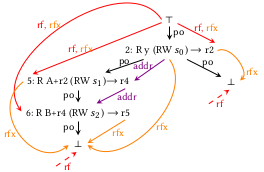
\includegraphics[width=0.6\linewidth]{lcm1}
	\caption{LCM without speculation, from \cite{mosier2022}}
  \label{fig:lcm1}
\end{figure}
\begin{figure}[t]
  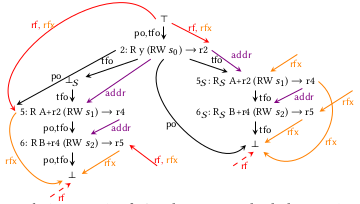
\includegraphics[width=0.8\linewidth]{lcm2}
	\caption{LCM with speculation, from \cite{mosier2022}}
  \label{fig:lcm2}
\end{figure}

Figure \ref{fig:lcm2} is a model of the same program with speculative execution.
This model now has edges labelled \texttt{tfo} for \emph{transient flow order} which complement \texttt{po} edges after a branch.
They represent program flow when a speculation is incorrect.
On the left side of the graph, there is a \texttt{tfo} edge leading to $\bot$, that is a branch to line 8 of the pseudo code is incorrectly speculated.
Then another \texttt{tfo} leads back to the line 5 instruction, that is recovering from the mistake and resuming \texttt{po}.
Now, on the right side of figure \ref{fig:lcm2} we see the microarchitectural state changes occurring along \texttt{tfo} paths and conclude that leakage is possible with this piece of code in a speculative environment.

\subsection{Bounded Model Checking}

Another proposal for modelling software to identify vulnerabilities is given in Ponce-de-León and Kinder's \textit{Cats vs. Spectre: An Axiomatic Approach to Modeling Speculative Execution Attacks}\cite{cats2022}.
The idea is to transform a given program into sets of relations and to specify constraints on program execution, both defined using Algave, Cousot, and Maranget's CAT language\cite{alglave2016syntax} and perform Bounded Model Checking\cite{biere2021BoundedMC} to (hopefully) achieve the desired result.
Bounded Model Checking is a search for a counterexamples to a model in executions of a program, bounded by some total number of executions.
Ponce-de-León and Kinder showed how to model execution constraints using CAT to identify a few Spectre variants in example snippets of code and implemented Bounded Model Checkers.
They then ran several benchmark programs through the resulting tool and compared the accuracy and performance against Spectector and Binsec. 
In order to achieve guarantees, Ponce-de-León and Kinder follow ``always mispredict semantics'' which forces the model checker to inspect the worse case for any predictor.

\begin{figure}[t]
  \centering
  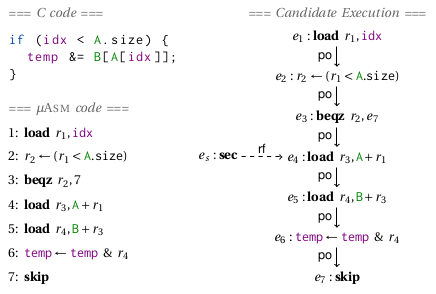
\includegraphics[width=0.9\linewidth]{cats1}
	\caption{Spectre-V1 vs. CATs reproduced from \cite{cats2022}}
  \label{fig:cats1}
\end{figure}

In Figure \ref{fig:cats1}, directly from \cite{cats2022}, we see the familiar Spectre gadget code snippet in C, translated to an assembly language, and then illustrated in the candidate execution graph where $e_3$ is mispredicted.
That is, \texttt{idx} is in fact greater than or equal to \texttt{A.size}, but the misprediction leads to executing $e_4$ which reads from \texttt{A} + \texttt{idx} which is out of bounds and can reach some memory location previously written to by $e_s$, where $e_s$ is some instruction handling a sensitive value.
The intuition here is that if we are predicting that $e_3$ is not going to take the branch, then the order in which $e_3$ and $e_4$ are retired does not matter, and so, in effect, the processor has reordered these instructions to conceal the delay of the read.
Placing a fence between these instructions prevents reordering and CAT can be used to show that such a revised program would be safe.

\begin{figure}[t]
  \centering
  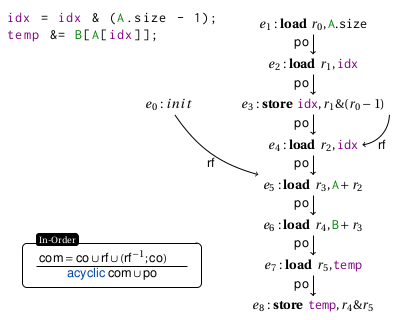
\includegraphics[width=0.9\linewidth]{cats2}
	\caption{A safe array access under in-order semantics reproduced from \cite{cats2022}}
  \label{fig:cats2}
\end{figure}

In figure \ref{fig:cats2} the program is revised to use \emph{index masking} to avoid the possibility of a branch misprediction instead of a fence.
The idea is that this would allow the processor to avoid stalling due to a fence.
The inset is a CAT description of the execution model.
\texttt{com} is defined as the set of relations of \emph{coherence order} (\texttt{co}) unioned with the set of \emph{reads-from} (\texttt{rf}) relations unioned with the composition of \texttt{rf\textsuperscript{-1}} with \texttt{co}.
The constraint that the graph formed by \texttt{com} unioned with the set of program order \texttt{po} relations is acyclic describes the execution behavior of an in-order processor with or without branch speculation.

Coherence order relates instructions that write to the same location, in program order.
Reads-from relates instructions that read from a memory location to the instruction which wrote the value that will be read.
Note that many of the \texttt{rf} relations are omitted from the diagram for clarity, according to the authors.
\texttt{rf\textsuperscript{-1}} is the set of inverse relationships of reads-from, that is it relates writes to the reads that access the written value.
Since there are no branch speculations, this access is safe under these constraints.

However, with the addition of store-to-load forwarding, it is possible to reorder $e_3$ and $e_4$, that is we can begin execution of $e_4$ before $e_3$ is complete.
That means that \texttt{idx} in both instructions proceed with the initial value -- a sort of misprediction that the store will alias the existing value\footnote{
	We struggled to understand this.
	However, it may help to realize that with store-to-load, the processor must guess something.
	In fact the paper later describes a model where the misprediction was that the value would \emph{not} be aliased and led to another version of the attack.
	We think.
}.
Figure \ref{fig:cats3} illustrates the salient relations now present in the program where store-to-load semantics are allowed.
Note that this graph would violate the constraint of the previous model of \texttt{com} $\cup$ \texttt{po} being acyclic, as there is a cycle $e_4\xrightarrow{rf^{-1}}e_0\xrightarrow{co}e_3\xrightarrow{po}e_4$.
Again, adding a fence between $e_3$ and $e_4$ can be shown to be safe with the additional relaxation of constraints need to accommodate store-to-forward.

\begin{figure}[t]
  \centering
  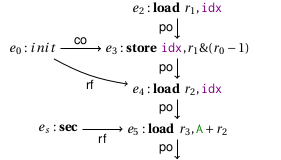
\includegraphics[width=0.6\linewidth]{cats3}
	\caption{Code snippet from figure \ref{fig:cats2} with store-to-load semantics reproduced from \cite{cats2022}}
  \label{fig:cats3}
\end{figure}



Future work based on this research could be to investigate application of CAT and Kaibyo to other speculative execution vulnerabilities.
The paper assumes a predictor that is incorrect every time, which would be the worse case scenario for speculative attacks.
There may be a way to show that predictor accuracy will affect the degree to which code is vulnerable to these kinds of attacks.



\section{Future Work}\label{sec:future}

Canella et al's success in classifying attacks which led to identifying additional variants gives us hope that a similar effort with respect to the defenses might yield additional defenses that might prove useful against future variants.
We believe there is opportunity both in expanding their classification system in the details and consolidating common features across attack variants.
There is significant overlap in their categories C2 and D2 and there are overlaps in C3 and D1.
An overarching trifurcation of approaches, subdivided on perhaps hardware vs software solution, might prove useful in identifying gaps in defense research.
For example, is there value in identifying ways to reduce the accuracy of data leaked to a Meltdown attack?

\section{Conclusion}
Summarize and incite.

Shepard, Brookes, and Denz \cite{shepherd2022transient} mention power consumption and EM radiation as potential side channels.
Could be sad sad how to axiomatic model \emph{all} side effects.
They also brought my attention to the fact that cache by itself presents a side channel with or without speculative execution.
Since caching can affect access speed in either case, a sufficiently precise timer can detect which cache lines have been recently touched and from there make inferences about values.
This is possible because addresses are the same thing as data - one can use data as an address and thereby affect cache state in a manner directly correlated to the data value.

Something about optimize for the common case.
Transient execution exploits the edges.
Can coin flips provide security and an acceptable performance?
Complicated machinery in processors to make predictions, throw predictions out and take an 80\% hit to performance.
But, replace them with highly/suffficiently rng, and make coin-flip predictions - 50\% of the time they're right every time?
Adds a ton of noise to the side channels, how much does it really affect performance from a non-speculative baseline or from the super advanced but exploitable current gen?

Lawl, I don't really want to pursue that, do I?
Would be hilarious, I think.

In Ponce-de-León and Kinder\cite{cats2022}, the reference another work about assume always mispredict and you can render security guarantees.
Could we show a tighter bound by means of coin flips?


\bibliographystyle{ieeetr}
\bibliography{paper}
\end{document}

